\documentclass[11pt]{article}
\usepackage[margin=1in]{geometry}
\usepackage[T1]{fontenc}
\usepackage[utf8]{inputenc}
\usepackage{hyperref}
\usepackage{graphicx}
\usepackage{enumitem}
\usepackage{xcolor}

\hypersetup{
  colorlinks=true,
  linkcolor=black,
  urlcolor=blue,
  citecolor=black
}

\title{Constellations: Low-Friction Exploratory Navigation with Evidence-Backed Bipartite Graphs}
\author{John Dimm\\Lean Software Development}
\date{Draft for discussion}

\begin{document}
\maketitle

\begin{abstract}
People often explore knowledge not only to answer a specific question, but to follow curiosity across many possible directions with minimal commitment: quickly trying an expansion, backing up, and trying another. We present \textbf{Constellations}, an interactive system for \textbf{low-friction exploratory navigation} that constructs \textbf{bipartite (Atomic--Composite)} graphs on demand from natural-language queries. Users begin with a single entity and iteratively expand the graph while the system enforces bipartite alternation. To reduce instability from mid-graph ontology drift, Constellations selects a bipartite pair from the first query (currently among Person--Event, Ingredient--Recipe, Symptom--Disease) and \textbf{locks it for the session} (no switching). To support interpretation and trust, Constellations attaches \textbf{evidence-backed edges} (short snippets with source links) so users can inspect the claimed reason behind a connection at any step. We describe the system design, position it relative to work on two-mode/affiliation networks and event-centric cultural heritage modeling, and outline an evaluation plan focused on recall, discovery, and sensemaking during iterative exploration.
\end{abstract}

\section{Introduction}
People often explore knowledge not to answer a single query, but to follow curiosity across many possible directions with minimal commitment: expand something, see what appears, and backtrack quickly to try a different branch. We call the boundary this process reveals the \textbf{knowledge frontier}---the set of adjacent ideas that are reachable from a current concept but not yet part of one's active memory. Interfaces for search, browsing, and encyclopedic reading support directed lookup, but can be less suited to this low-friction, branching process of ``what else is nearby?'' where the cost of trying a path is intentionally small.

Constellations is designed for this mode. Starting from a single user-provided entity, the system constructs a small, local graph and supports repeated \textbf{expand} operations that reveal additional connected entities. The key design decision is to enforce a \textbf{bipartite alternation constraint}: nodes alternate between \textbf{Atomic} entities (individuals or elementary concepts) and \textbf{Composite} entities (events, works, groups, conditions, or other aggregations). This constraint yields a stable interaction model across domains: atomic nodes are expanded into composites, and composites into atomics.

Because the system operates in open-world settings and aims for broad domain coverage, Constellations uses a large language model (LLM) to propose candidate neighbors during expansion. However, exploratory systems that rely on generative models face an interpretability challenge: users naturally ask \textbf{why} a connection exists before deciding whether it is worth pursuing. To address this, Constellations attaches \textbf{edge evidence}: short evidence snippets and source links displayed when an edge is selected. Evidence is treated as support for interpretation and verification, not as proof of causal claims.

\paragraph{Kiosk-first exploration.}
Constellations includes a kiosk mode (default) designed for touch displays and public installations: users start from curated seeds (no typing) and drive exploration by tapping nodes. When multiple bipartite pairs are enabled, the system chooses a pair from the first query and locks it for the session to reduce mid-graph drift.

\section{Related Work}
Constellations sits at the intersection of (1) sensemaking-oriented visualization and interactive graph exploration, (2) two-mode / affiliation networks and event-centric modeling, and (3) LLM-mediated interfaces that must communicate uncertainty and evidence.

\subsection{Two-mode / affiliation networks}
Two-mode (bipartite) networks are a long-standing model for situations where actors participate in events or belong to groups (e.g., actors--movies, authors--papers). A key methodological lesson is that naive projection into one mode can introduce artifacts; bipartite structure deserves analysis and visualization in its own right.

\subsection{Event-centric cultural heritage modeling}
Event-centric cultural heritage modeling emphasizes events as connective tissue relating people, places, objects, and documents. Constellations is aligned with this frame in its origin domain (people--events), and extends it across domains by choosing an Atomic--Composite pairing for the seed term.

\subsection{Positioning}
Constellations can be read as a synthesis of progressive disclosure in node-link exploration, the representational clarity of affiliation networks, and open-world neighbor proposal via an LLM. It emphasizes rapid branching and backtracking, and foregrounds interpretability at the granularity where exploration decisions are made: the edge. Compared to free-form LLM browsing, Constellations introduces stabilizers (bipartite alternation and a session-level lock of the Atomic--Composite pair chosen from the seed) to reduce drift and preserve coherent local structure.

\section{System}
\subsection{Overview}
Constellations constructs a small, local graph from a seed entity and supports repeated expansion. The system enforces a bipartite alternation constraint:
\begin{itemize}[leftmargin=*]
  \item \textbf{Atomic nodes}: individual entities or elementary concepts (e.g., Person, Ingredient, Symptom).
  \item \textbf{Composite nodes}: aggregations, works, events, groups, or conditions that connect multiple atomics (e.g., Movie, Recipe, Disease, Historical Event/Incident).
\end{itemize}

\subsection{Data flow}
\begin{enumerate}[leftmargin=*]
  \item \textbf{User query}: in kiosk mode (default), the user taps a curated seed; in non-kiosk mode, the user can type a query.
  \item \textbf{Context retrieval}: fetch lightweight context (e.g., Wikipedia summary) to help disambiguation and mitigate model knowledge gaps.
  \item \textbf{Start-pair classification (locked)}: choose a bipartite pair from the first input (currently one of Person--Event, Ingredient--Recipe, Symptom--Disease), then lock it for the session.
  \item \textbf{Expansion}: call the LLM to propose neighbors on the opposite partition, conditioned on the locked pair.
  \item \textbf{Evidence attachment}: each neighbor includes an evidence snippet and a source page title/URL; selecting an edge reveals evidence.
  \item \textbf{Caching}: store nodes and edges (with evidence) to reduce repeated calls and support persistence.
\end{enumerate}

\subsection{Figures}
\begin{figure}[h]
  \centering
  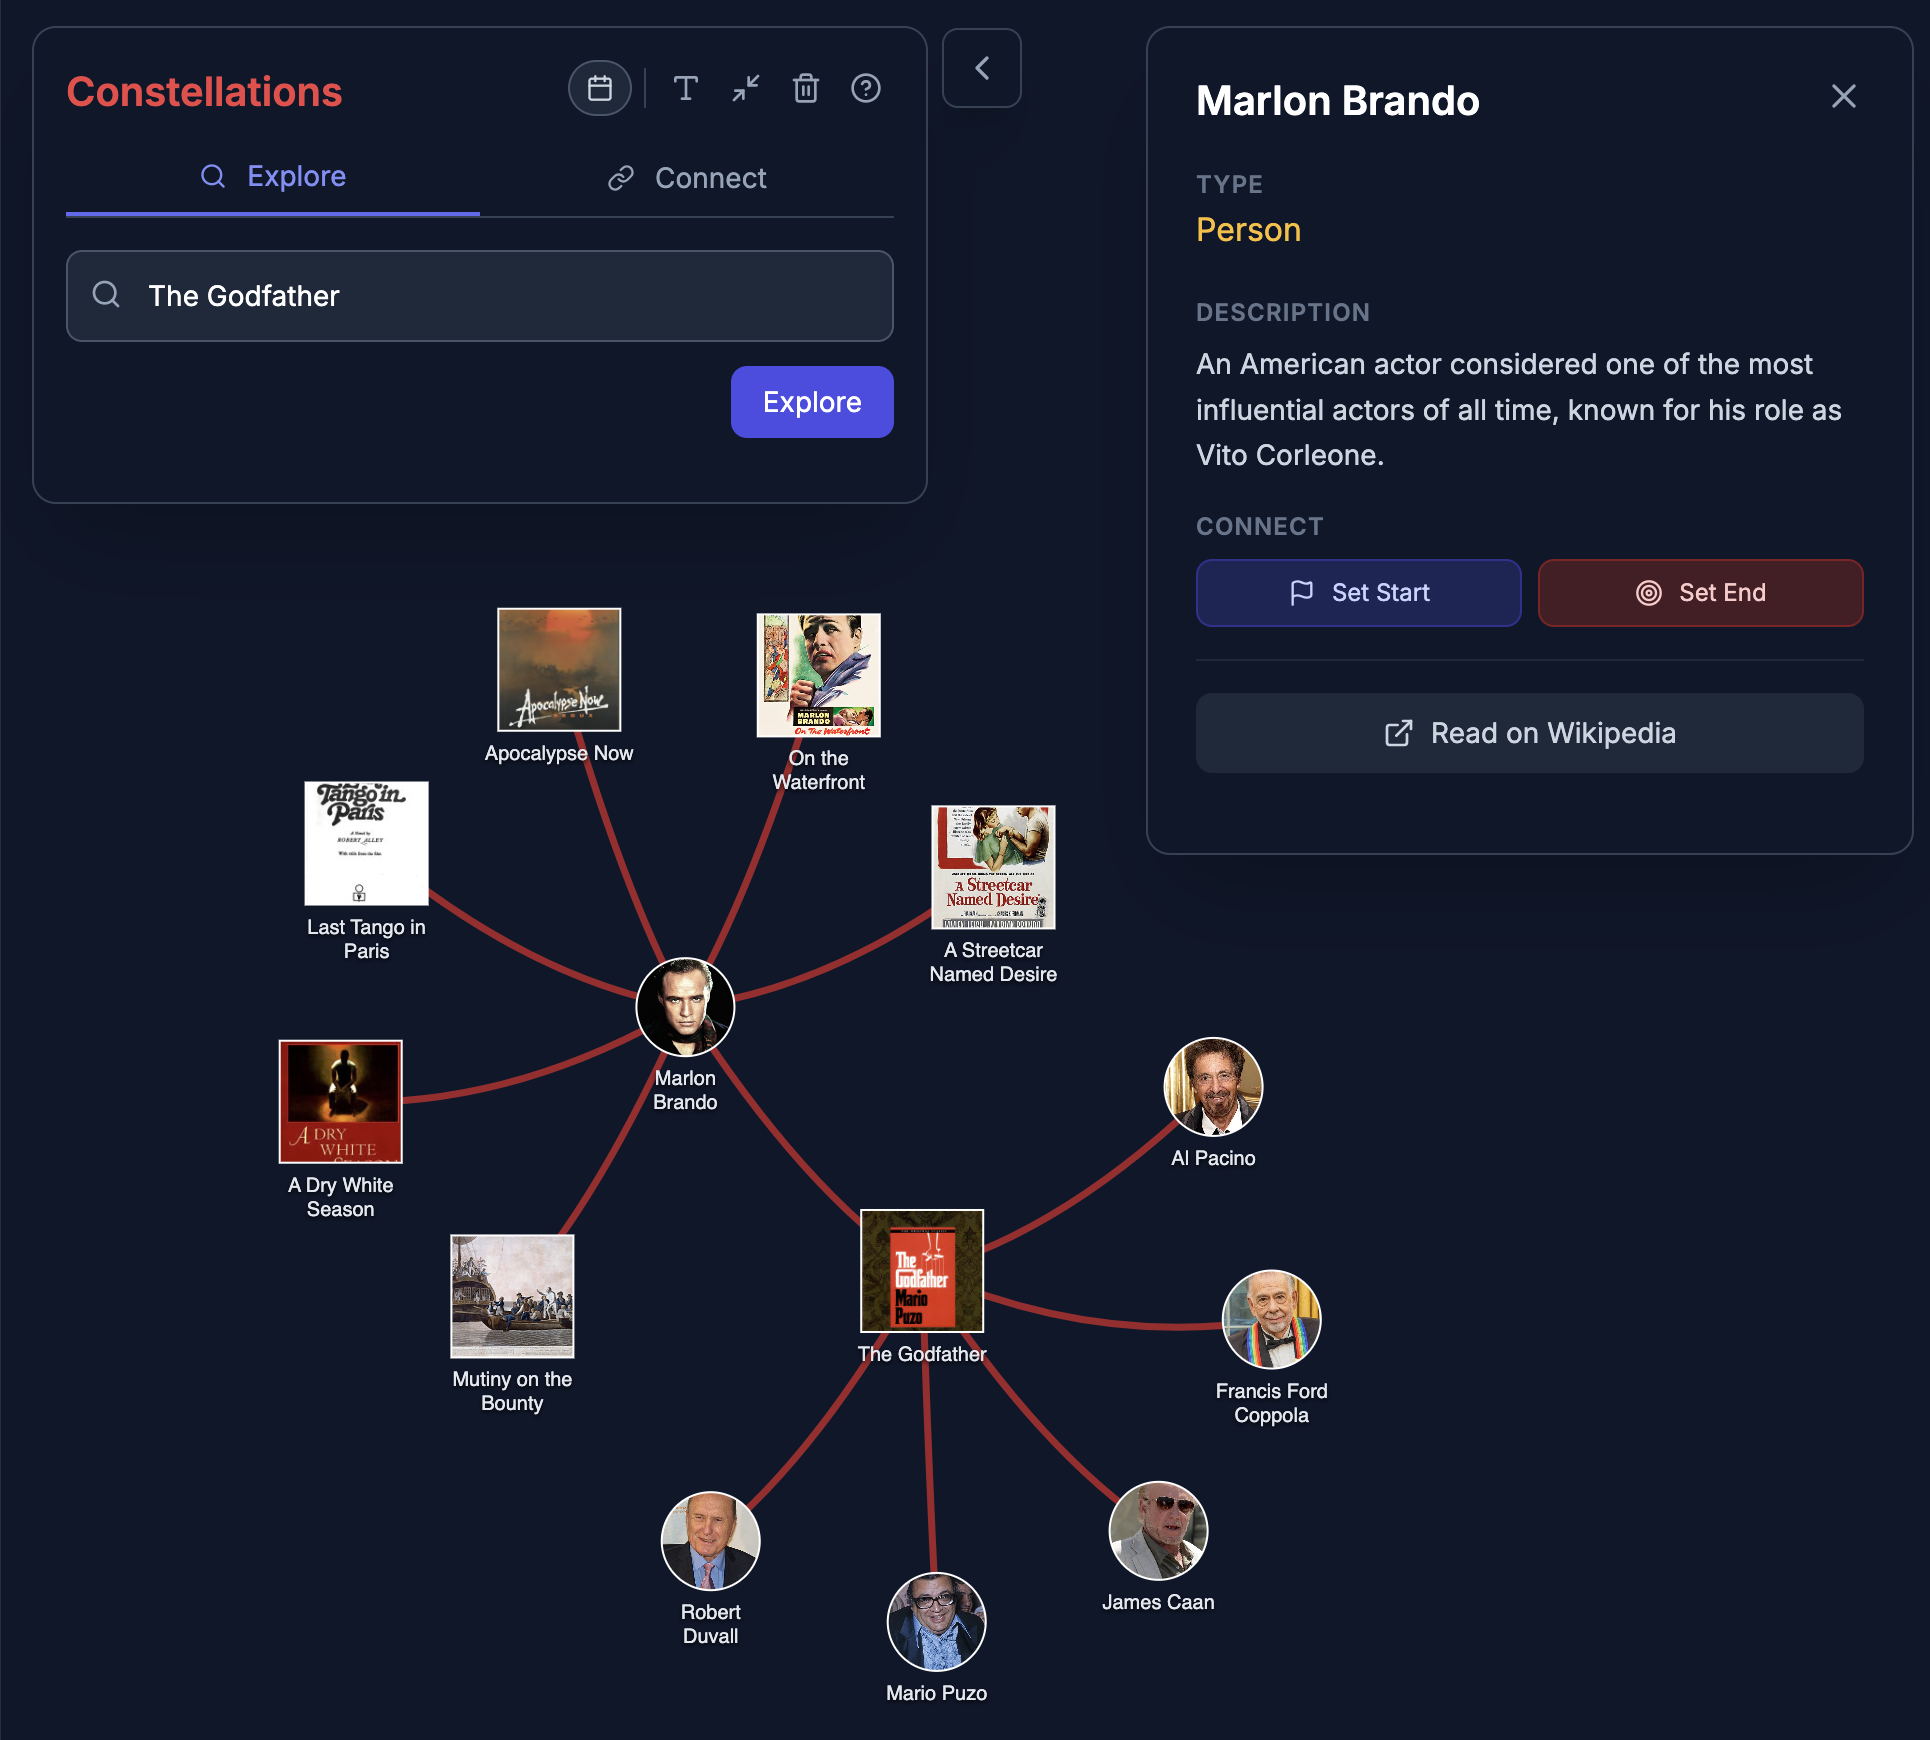
\includegraphics[width=0.60\linewidth]{../../godfather-brando.png}
  \caption{The Godfather expansion (screenshot).}
\end{figure}

\begin{figure}[h]
  \centering
  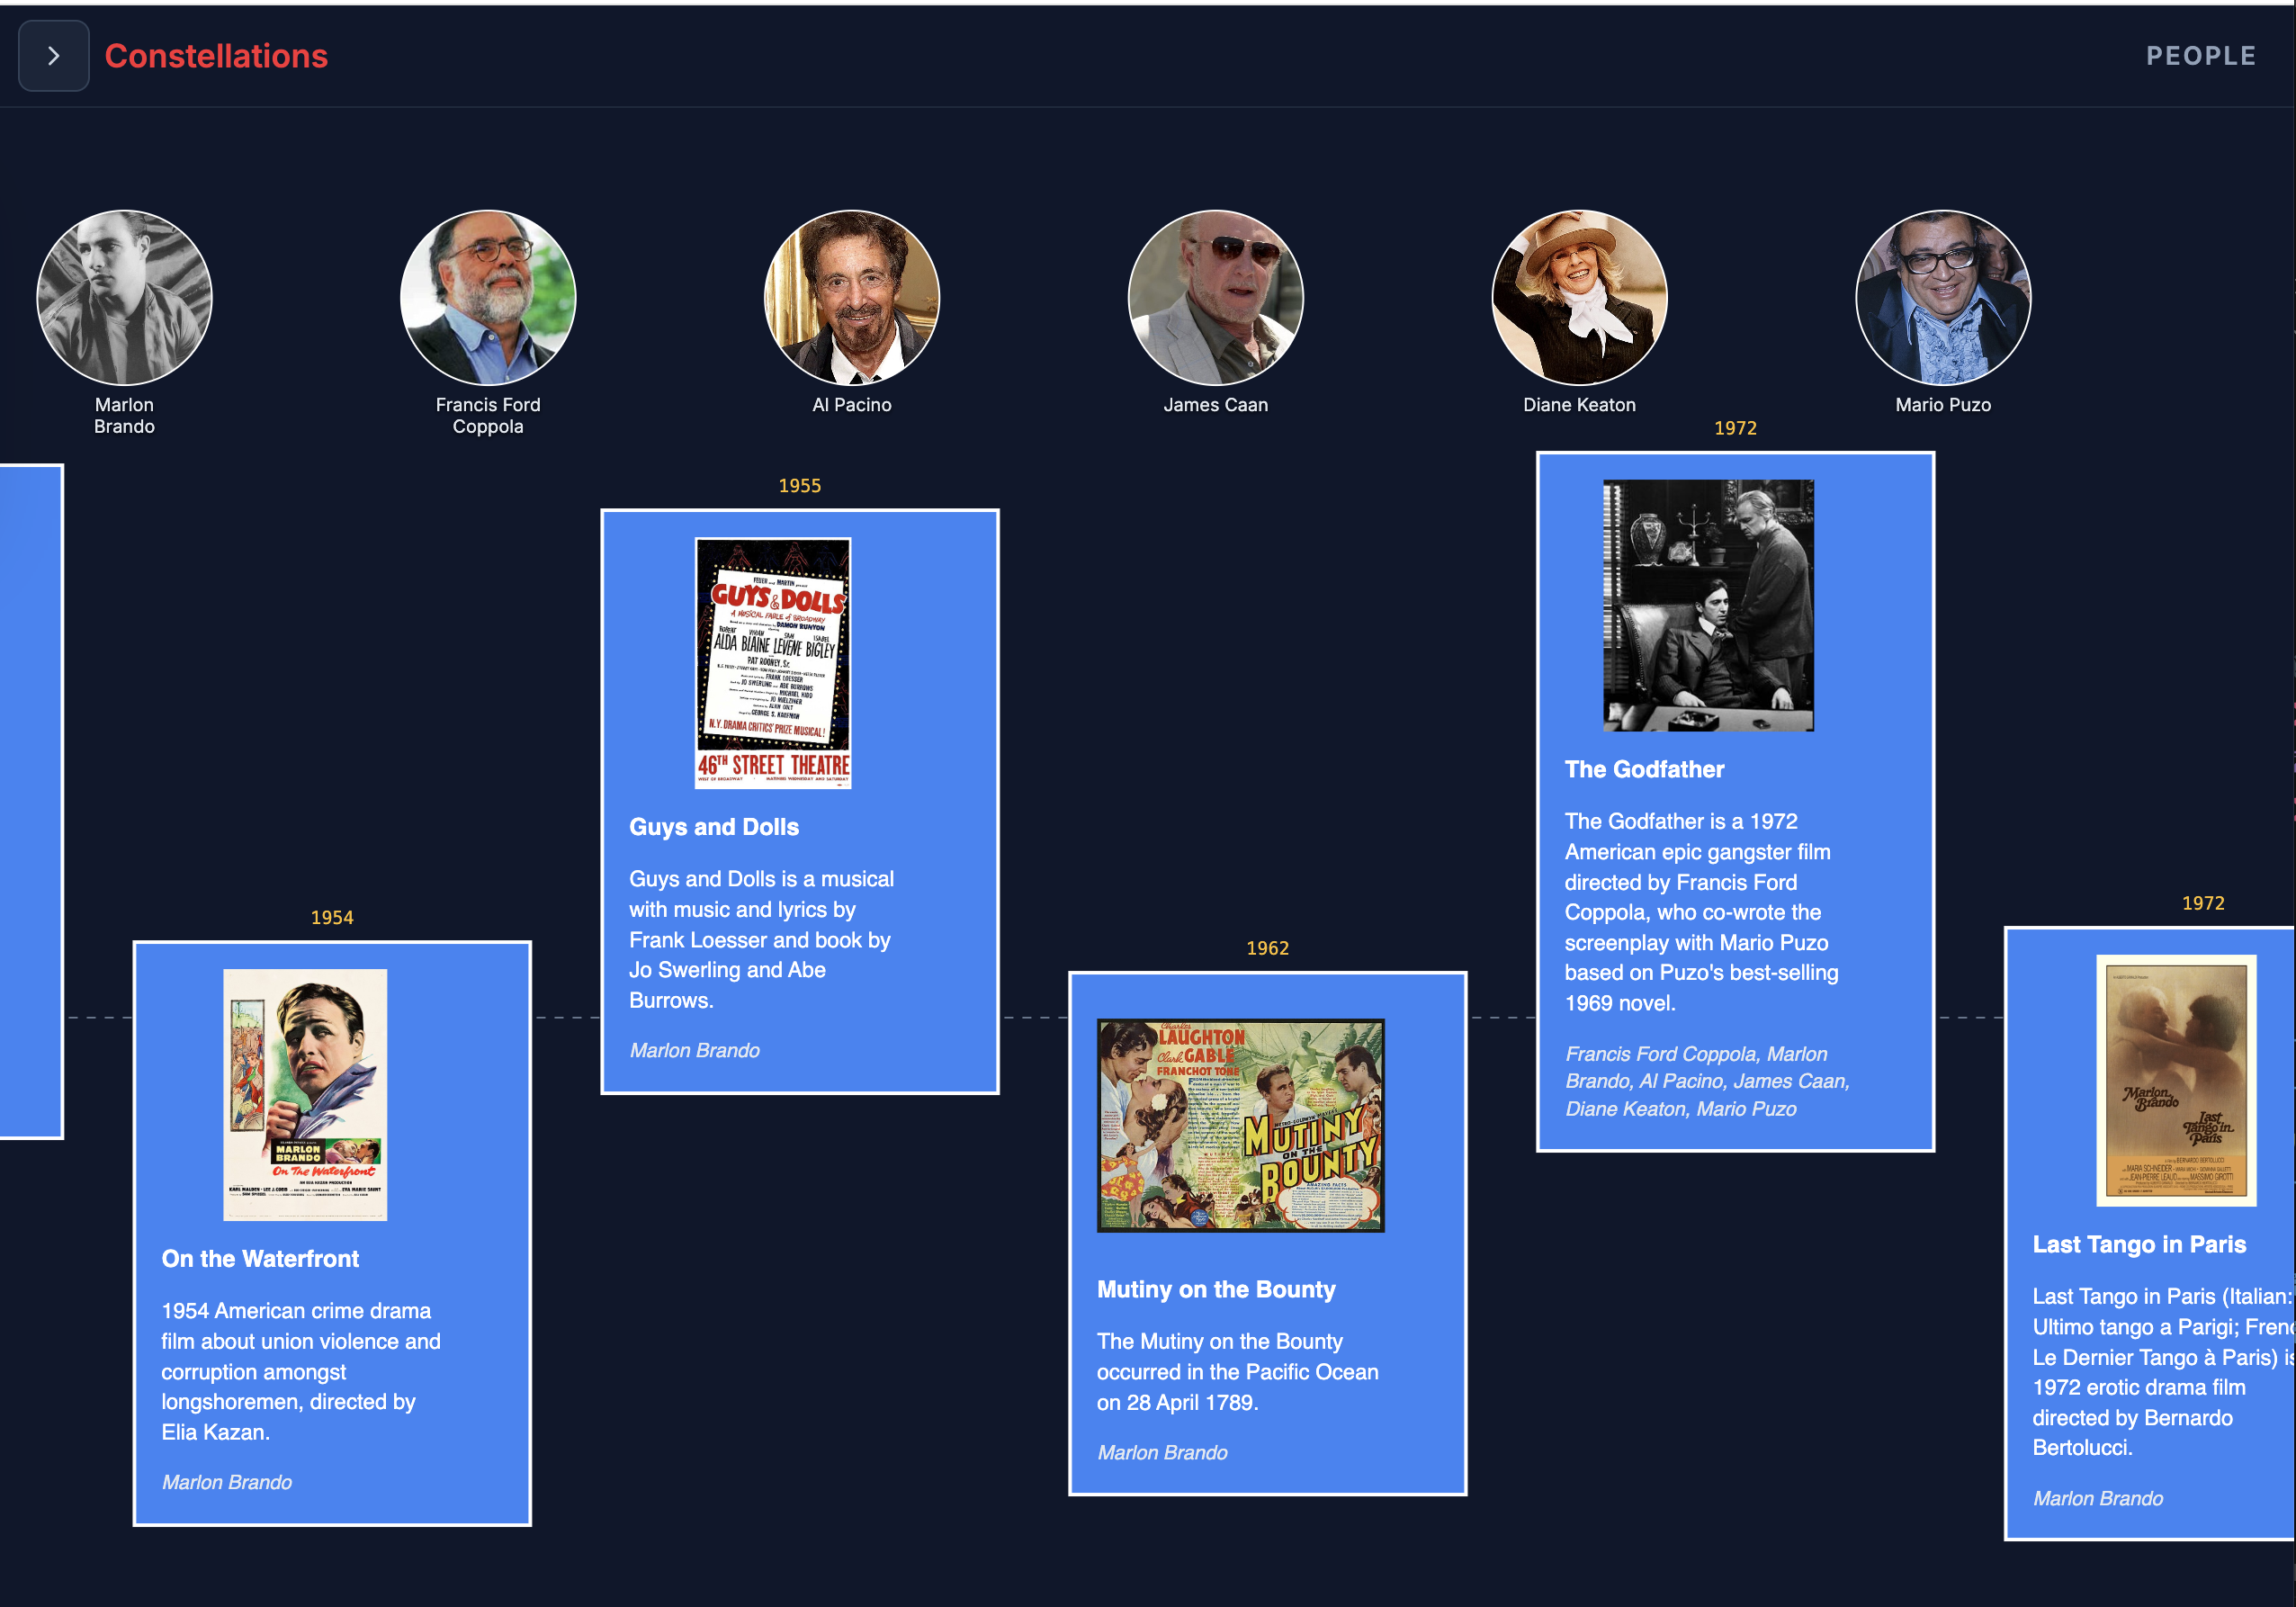
\includegraphics[width=0.60\linewidth]{../../godfather-timeline.png}
  \caption{Timeline view example (screenshot).}
\end{figure}

\section{Evaluation Plan}
We outline a mixed-method evaluation aligned with low-friction branching exploration rather than accuracy alone.
\begin{itemize}[leftmargin=*]
  \item \textbf{Study 1 (task-based)}: recall, discovery, frontier navigation, and evidence-use tasks; compare evidence on/off and (when applicable) pair-locking on/off; measure time, steps, backtracks, perceived orientation, and qualitative frontier moments.
  \item \textbf{Study 2 (offline)}: neighborhood quality proxies (named-entity quality, diversity, evidence availability, stability across repeated runs).
\end{itemize}

\section{Discussion and Future Work}
\subsection{Limitations}
Open-world ambiguity, recency gaps, and uneven evidence quality remain key challenges. Session-level pair locking reduces drift but can constrain legitimate cross-type exploration. Force-directed layouts work well for small neighborhoods but can degrade under repeated bulk expansion.

\subsection{Future work}
Promising directions include bipartite-aware expansion ranking, stronger evidence and provenance (multi-snippet and verification), ``soft locks'' for pair selection, curated domain packs for public installations, and multi-resolution views for scaling.

\section*{References (working list)}
\begin{thebibliography}{9}
\bibitem{heer2012}
Heer, J., \& Shneiderman, B. (2012). Interactive Dynamics for Visual Analysis. \url{https://idl.cs.washington.edu/papers/interactive-dynamics/}

\bibitem{brehmer2013}
Brehmer, M., \& Munzner, T. (2013). A Multi-Level Typology of Abstract Visualization Tasks. \url{https://doi.org/10.1109/TVCG.2013.124}

\bibitem{borgatti}
Borgatti, S. P. Network Analysis of Two-Mode Data. \url{https://www.researchgate.net/profile/Stephen-Borgatti/publication/222212892_Network_Analysis_of_Two_Mode_Data/}

\bibitem{faust2005}
Faust, K. (2005). Using Correspondence Analysis for Joint Displays of Affiliation Networks. \url{https://sites.socsci.uci.edu/~kfaust/faust/research/articles/faust_correspondence_analysis_2005.pdf}

\bibitem{wikidata}
Vrande\v{c}i\'{c}, D., \& Kr\"{o}tzsch, M. (2014). Wikidata: A Free Collaborative Knowledge Base. \url{https://doi.org/10.1145/2629489.2629492}
\end{thebibliography}

\section*{Acknowledgements / Author Note}
\textbf{Author.} John Dimm, Lean Software Development (sole proprietorship). Degrees from the University of Washington. Previously worked for 9 years in the Advanced Technology Group at Encyclopaedia Britannica.

\textbf{AI assistance.} This draft and the Constellations software were developed with assistance from large language models (LLMs) used as a programming and writing aid (e.g., generating code suggestions, outlining text, and editing prose). The LLM is not an author and does not take responsibility for the content.

\textbf{Media and data sources.} Node summaries and many images are drawn from Wikipedia and Wikimedia Commons. Any errors or omissions in how sources are attributed are the author's responsibility.

\end{document}

